\section{Partie 3:Etude de performance et optimisations}
\paragraph{}Je me suis finalement penché sur les performances de la version 3D de NTMIX développé au cours de ce stage. J'ai dans un premier temps étudié les performances séquentielles du programme (code tel qu'il était à la fin de la première partie) puis les performances de la version parallèle.
\subsection{Présentation du matériel}
L'ensemble des tests suivants ont été réalisés sur les calculateurs internes du CERFACS, le Bullx B510 (neptune) et le LENOVO (nemo). Ils possèdent les caractéristiques suivantes:

\begin{table}[h]
  \begin{center}
    \begin{tabular}{|M{3.5cm}|M{5cm}|M{5cm}|}
      \hline
      & Neptune & Nemo \\
      \hline
      Noeuds & 158 & 252 \\
      \hline
      Puissance crête & 53 TFlop/s & 242 TFlop/s \\
      \hline
      Consommation maximale applicative & 51 kW.h & 73 kW.h \\
      \hline
      Consommation à vide & 25 kW.h & 34 kW.h \\
      \hline
      Processeurs & Intel Sandy Bridge 8 coeurs (2.6 GHz) & Intel Ivy bridge 12 coeurs (2.5 GHz) \\
      \hline
      Mémoire & 32 Go de mémoire cadencée à 1.6 GHz & 64 Go de mémoire cadencée à 2.1 GHz \\
      \hline
    \end{tabular}
  \end{center}
  \caption{\label{tab:carac}Caractèristiques des calculateurs du Cerfacs}
\end{table}

\begin{figure}[ht]
  \centering
  \begin{minipage}{.5\textwidth}
    \centering
    \includegraphics[width=.7\linewidth]{figures/neptune.jpg}
    \caption{\label{fig:neptune}Neptune}
  \end{minipage}%
  \begin{minipage}{.5\textwidth}
    \centering
    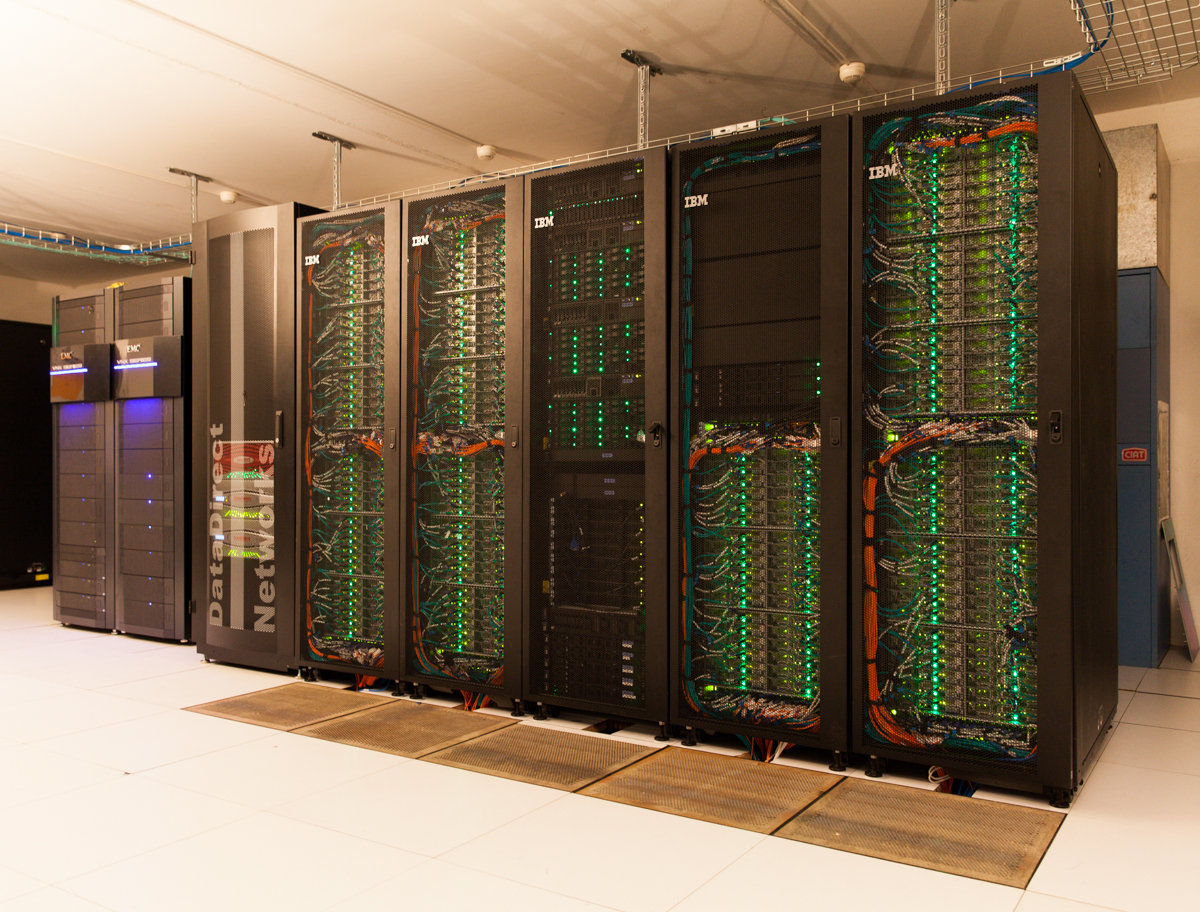
\includegraphics[width=.9\linewidth]{figures/nemo.jpg}
    \caption{\label{fig:neptune_node}Nemo}
  \end{minipage}
\end{figure}



\subsection{Performances séquentielles}
Une fois le programme testé et fonctionnel, j'ai commencé à étudier ses performances. J'ai, dans un premier temps, mesuré un temps de référence pour l'exécution de ce programme; compilation par défaut, donc avec l'option -O2.

\subsubsection{Vectorisation}
J'ai ensuite compiler le programme avec l'option -xAVX qui permet de générer un code vectorisé pour les processeurs possédant l'extension AVX. Pour profiler le programme, j'ai utilisé Intel Advisor qui permet d'analyser la vectorisation d'un programme. Comme on peut le constater sur la figure \ref{fig:advixe}, le compilateur n'a vectorisé qu'un faible pourcentage de boucles (en comparaison avec la référence cf img). Ceci vient du fait que l'ensemble des variables sont contenues dans un unique tableau (fig. \ref{fig:array_s}) et qu'on y accède grâce à des pointeurs. Lorsqu'une boucle doit travailler sur plusieurs tableaux contenus dans ce grand tableau (fig. \ref{fig:o2_avx_novect}), le compilateur assume qu'elle travaille sur un unique grand tableau et empêche donc la vectorisation au profit de la cohérence. Pour résoudre ce problème, il suffit d'indiquer au compilateur qu'il n'y a pas aliasing; on garantit ainsi qu'une zone mémoire ne peut être accédée que par un nom et que le programme ne dépassera pas les limites d'un tableau.


\begin{figure}	
  \centering
  \begin{minipage}{.5\textwidth}
    \centering
    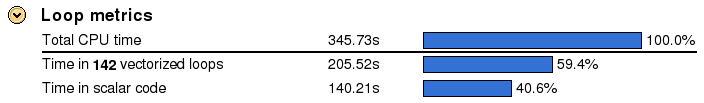
\includegraphics[width=.9\linewidth]{figures/advixe_O2.png}
    \caption{\label{fig:advixe_o2}}
  \end{minipage}%
  \begin{minipage}{.5\textwidth}
    \centering
    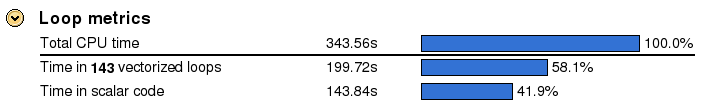
\includegraphics[width=.9\linewidth]{figures/advixe_O2_avx.png}
    \caption{\label{fig:advixe_o2_avx}Caption 2}
  \end{minipage}
  \caption{Répartition des boucles}\label{fig:advixe}
\end{figure}

\begin{figure}[ht]
  \centering
  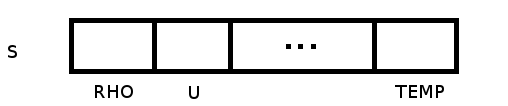
\includegraphics[scale=0.35]{figures/array_s.png}
  \caption{\label{fig:array_s}Structure de la mémoire}
\end{figure}


\begin{figure}[h]
  \centering
  \begin{lstlisting}
    !
    !    DETERMINE THE MASS FRACTION
    !
    DO I=1,NX*NY*NZ
    YK(I)=RHO_Y_TILDE(I,K)/RHO(I)
    END DO
  \end{lstlisting}
  \caption{\label{fig:o2_avx_novect}Boucle non vectorisée}
\end{figure}



\begin{figure}	
  \centering
  \begin{minipage}{.5\textwidth}
    \centering
    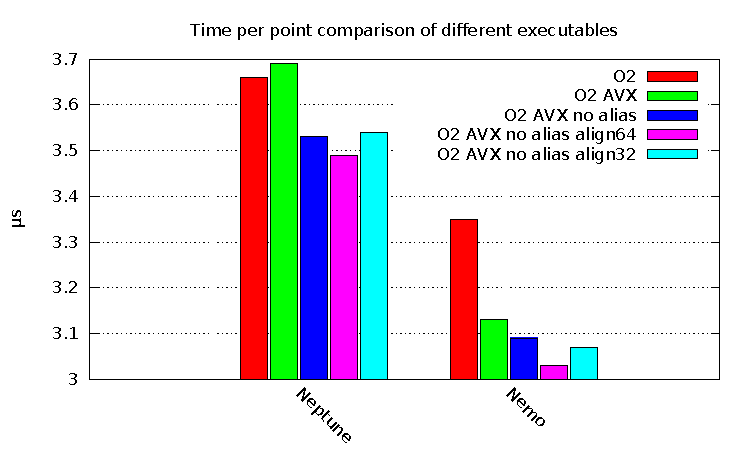
\includegraphics[width=.9\linewidth]{gnuplot/bench_scalaire_per_compute.pdf}
  \end{minipage}%
  \begin{minipage}{.5\textwidth}
    \centering
    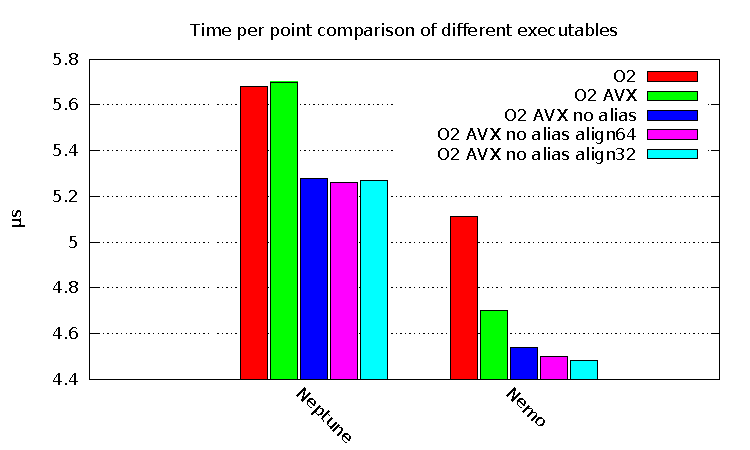
\includegraphics[width=.9\linewidth]{gnuplot/bench_scalaire_per_diag.pdf}
  \end{minipage}
  \caption{Temps par point - Cas périodique}\label{fig:scal_tpp}
\end{figure}


\begin{figure}	
  \centering
  \begin{minipage}{.5\textwidth}
    \centering
    % \includegraphics[width=.9\linewidth]{gnuplot/bench_scalaire_sym_compute.pdf}
    \caption{\label{fig:scal_compute}}
  \end{minipage}%
  \begin{minipage}{.5\textwidth}
    \centering
    % \includegraphics[width=.9\linewidth]{gnuplot/bench_scalaire_sym_diag.pdf}
    \caption{\label{fig:scal_diag}Caption 2}
  \end{minipage}
  \caption{Temps par point - Cas symétrique}\label{fig:scal_tpp}
\end{figure}



\subsubsection{Alignement de la mémoire}
blabla marche pas

\paragraph{durée=f(taille)}


\subsection{Performances parallèle}

\subsubsection{Méthode de recouvrement}



\subsubsection{Méthode de communication}
